% !TeX root = ../thesis.tex

\section{Introduction}
Chapter~\ref{ch:dispvit} showed that a single Transformer stream can encode semantic context and binocular geometry from a stereo pair.
This result advances the thesis from explicit stereo matching toward unified static geometry representation, but robotic perception rarely ends at a fixed stereo pair.
A robot receives a video stream and needs two kinds of geometry at different time scales: transient per-frame depth for immediate reaction, and consolidated keyframe depth and motion for a coherent local map.
Temporal observations provide motion parallax beyond static stereo, yet they also entangle depth, ego-motion, dynamic objects, optical-flow reliability, and monocular scale.
The final technical step of this thesis is therefore to move from unified static representation to a temporal representation that can operate inside a streaming local-mapping runtime.

The most established route to video geometry is to optimize camera motion and scene structure through SfM or SLAM.
Classical systems optimize reprojection or photometric residuals over visual measurements~\cite{schoenberger2016sfm,murAcceptedTRO2015}, while neural systems strengthen this paradigm by embedding dense bundle adjustment (DBA) into learned update networks, as in DROID-SLAM~\cite{teed2021droid}, and by adding monocular depth priors and dynamic-region weighting, as in MegaSaM~\cite{li2025megasam}.
These methods are highly effective for pose and trajectory estimation, but their central optimization target is not the same as the one studied in this chapter.
In MegaSaM, for example, the final video depth is obtained through a separate offline video-depth optimization procedure rather than being simply the online BA state.
This difference motivates a narrower formulation: GeoNT acts as a learned measurement layer for streaming local mapping, with immediate tracking depth for the current frame, keyframe-aligned depth for selected keyframes, and scale-normalized pose measurements that a lightweight graph can use for local consistency.

Recent feed-forward geometry Transformers offer a second tempting direction, but they do not by themselves solve the streaming local-mapping problem considered here.
Models such as DUSt3R~\cite{wang2024dust3r}, MASt3R~\cite{leroy2024grounding}, and VGGT~\cite{wang2025vggt} show that Transformer backbones can infer dense geometry, cameras, and correspondences from RGB views.
Their strength is global aggregation over visual input, often in an offline or batch multi-view setting.
When used directly in an online stream, however, such models can face a difficult operating point: the system must select keyframes, keep latency bounded, produce usable depth and motion before the whole sequence is available, and maintain local pose-scale consistency.
Monocular depth-prior systems address a different part of the problem: they provide strong single-image shape estimates, but the mapping system must still determine the metric gauge and temporal measurement policy.
Thus, the goal here is not to regress all geometry from appearance alone, nor to use a monocular prior as a final depth product.
The goal is to design a keyframe-based temporal measurement model around the geometric signals that monocular video already exposes.

This chapter studies that goal through \emph{GeoNT}, a Geometry-Native Transformer for streaming depth and motion estimation.
The central contribution is a geometry-native temporal representation that explicitly maps monocular video cues to local depth and motion measurements.
Given a monocular video stream with fixed intrinsics, monocular depth priors, and optical-flow estimates with reliability cues, GeoNT produces normalized depth for the reference frame or keyframe and reference-scale-normalized relative pose measurements to nearby support keyframes.
Within the keyframe-based local mapping formulation, transient estimates support online response, while selected keyframes define keyframe-aligned dense geometry and graph-compatible motion measurements after temporal support becomes available.
Instead of treating RGB appearance as the main token signal, GeoNT tokenizes optical flow, flow uncertainty, intrinsics-normalized rays, and a normalized monocular depth prior.
Optical flow describes the apparent motion between frames, intrinsics convert pixel displacement into camera-normalized motion, flow uncertainty indicates where this motion is reliable, and monocular depth supplies learned scene structure when parallax is weak.
GeoNT relates the current view, or a keyframe whose local temporal support is available, to a local set of support keyframes, predicting refined normalized depth and reference-scale-normalized relative pose measurements for keyframe-based mapping.
Architecturally, GeoNT separates dense geometry patch tokens from compact camera tokens: patch tokens carry local motion and depth evidence, while camera tokens provide a pair-level conditioning signal for interpreting motion.
Because this representation depends on reliable temporal correspondence, GeoNT also uses a flow frontend with ViT-based motion-basis initialization to support larger-baseline matching before Transformer aggregation.

The same formulation also sets the system boundary.
GeoNT does not include full SLAM, dense bundle adjustment, loop closure, relocalization, or dense geometry for every incoming frame.
This boundary motivates the current evaluation protocol, which focuses on keyframe-aligned depth under a consistent video-level scale and direct graph-factor quality for GeoNT relative-pose measurements.

Within the thesis narrative, GeoNT completes the progression from spatial and semantic geometry to temporal geometry.
The previous chapters move from stereo correspondence, to semantic-geometric alignment, to unified static representation.
GeoNT extends this line by replacing image-token reasoning with tokenized temporal motion, ray geometry, reliability, and monocular structure.
The representation is used in two estimation regimes.
During frontend tracking, an incoming frame receives a transient depth and relative motion estimate for low-latency response.
After keyframe selection, selected frames become keyframe nodes in the local map; once sufficient neighboring support keyframes are available, a single multi-view aggregation establishes their keyframe-aligned depth estimates and pose measurements for the pose-scale graph.
This distinction determines how GeoNT separates online response from keyframe-aligned local geometry.

The technical contributions of this chapter are summarized as follows.
\begin{itemize}[leftmargin=*]
    \item \textbf{Geometry-token measurement formulation.}
    The chapter formulates monocular video local mapping as Transformer reasoning over optical flow, flow uncertainty, intrinsics-normalized rays, and normalized monocular depth, rather than over RGB image tokens alone.
    \item \textbf{Camera-conditioned temporal aggregation.}
    GeoNT separates dense geometry patch tokens from compact camera tokens, uses adaptive camera-token conditioning to interpret flow-depth evidence, and predicts refined normalized depth together with reference-scale-normalized relative pose measurements.
    \item \textbf{Keyframe runtime and scale convention.}
    The runtime distinguishes transient per-frame tracking depth from keyframe-aligned depth, uses one temporally supported multi-view refinement for each selected keyframe, and inserts scale-normalized neural pose edges into a pose-scale graph whose node scales provide the metric interpretation of keyframe depth.
\end{itemize}
Together, these contributions complete the thesis progression from stereo correspondence and semantic context to temporal geometry, while keeping the system claim scoped to streaming local perception.

The rest of this chapter is organized as follows.
Section~\ref{sec:geont_problem} defines the temporal geometry problem and the depth-scale convention.
Section~\ref{sec:geont_model} describes the Geometry-Native Transformer.
Section~\ref{sec:geont_streaming} presents the streaming local mapping runtime.
Section~\ref{sec:geont_pgo} introduces the pose graph optimization objective.
Section~\ref{sec:geont_eval_protocol} describes the evaluation protocol and analysis dimensions.
Section~\ref{sec:geont_discussion} discusses the role and limitations of the system, and Section~\ref{sec:geont_conclusion} concludes the chapter.

\section{Problem Formulation}
\label{sec:geont_problem}

\subsection{Temporal Geometry from Monocular Video}
Streaming monocular mapping requires a representation that separates local scene shape, metric scale, and camera motion.
A single image can provide a strong relative scene-shape estimate through monocular priors, but its metric scale is not determined without temporal motion.
GeoNT therefore represents each keyframe $i$ with a camera pose $\bm{T}_i \in SE(3)$, a normalized depth map $\bm{D}_i$, and a positive metric scale $s_i$.
Given a monocular RGB video $\{\bm{I}_t\}_{t=0}^{T-1}$ with fixed camera intrinsics $\bm{K}$, the metric depth associated with keyframe $i$ is
\begin{equation}
    \bm{Z}_i = s_i \bm{D}_i .
    \label{eq:geont_metric_depth}
\end{equation}
This factorization assigns local scene geometry to the depth map and assigns metric calibration to the scalar scale.
The graph therefore adjusts the metric interpretation of a keyframe without changing the depth map itself.
The modeling assumption is that intrinsics and preprocessing are fixed over the stream, that a monocular depth prior is available for each frame, and that optical flow provides the explicit temporal correspondence cue from which GeoNT forms its measurements.

Temporal geometry is observed through inter-frame optical flow, but a flow field alone does not determine depth or relative camera motion uniquely.
We denote by $i$ the reference view whose depth is being estimated.
A temporal support keyframe $j$ provides the comparison view, and the optical flow from $i$ to $j$ measures where pixels in the reference view are observed in the support view.
If a pixel $\bm{x}=(u,v)$ in the reference view has depth $Z_i(\bm{x})$, the rigid flow induced by a relative pose $\bm{T}_{ji}=\bm{T}_j \bm{T}_i^{-1}$ is
\begin{equation}
    \bm{f}_{ij}^{\mathrm{rigid}}(\bm{x})
    =
    \pi\!\left(
        \bm{K}\bm{T}_{ji}
        \left[
        Z_i(\bm{x})\bm{K}^{-1}\bar{\bm{x}}
        \right]
    \right) - \bm{x},
    \label{eq:geont_rigid_flow}
\end{equation}
where $\bar{\bm{x}}=(u,v,1)^\top$ and $\pi(\cdot)$ denotes perspective projection.
Equation~\ref{eq:geont_rigid_flow} shows why depth and pose are coupled: the same observed flow can be explained by different combinations of translation, rotation, depth, and moving objects.
Degenerate motions make this coupling especially difficult.
Pure rotation provides little depth parallax, and near-forward translation produces small lateral displacement for many pixels.
Dynamic objects introduce flow that cannot be explained by a single static-scene camera motion.

GeoNT treats this ambiguity as a learned measurement problem over geometric cues.
Optical flow supplies direct evidence of inter-view correspondence, while a monocular geometry model supplies a normalized depth prior~\cite{wang2025moge2}.
Given a reference view and nearby support keyframes, GeoNT predicts a refined depth representation for the reference view together with relative pose measurements between the reference view and the support keyframes.
These outputs provide the quantities needed to explain the observed flow under the rigid-projection model: local scene shape and relative motion between views.
The GeoNT measurement is scale-normalized rather than metric: it does not output an independent scale, and its translation magnitude is interpreted relative to the normalized depth of the reference view.
The metric scale is introduced separately by the keyframe scale variable defined in the next subsection.

\subsection{Depth and Scale Convention}
The depth-scale convention separates neural scene-shape refinement from metric-scale optimization.
The reason is the monocular gauge ambiguity: if all depths and translations in a local monocular reconstruction are multiplied by the same positive constant, the induced image motion can remain unchanged.
The video therefore constrains the shape and relative motion more directly than it constrains the absolute metric unit.
GeoNT follows this structure by predicting depth in a normalized gauge and by letting the runtime attach a metric scale to each keyframe.

Let $\tilde{\bm{D}}_i$ denote the normalized monocular depth prior for keyframe $i$, and let $s_i^0$ denote its initial scale before graph optimization.
GeoNT inference uses $\tilde{\bm{D}}_i$ as the depth input, rather than feeding the current refined keyframe depth $\bm{D}_i$ back into the network.
This choice keeps each measurement anchored to the same monocular reference shape and avoids a feedback loop in which repeated neural updates drift away from the original geometric prior.

The refined depth map $\bm{D}_i$ represents the scene shape estimated for a reference keyframe, while the scalar $s_i$ gives its metric interpretation through Equation~\ref{eq:geont_metric_depth}.
The normalized prior $\tilde{\bm{D}}_i$ and the refined depth $\bm{D}_i$ therefore play different roles: the prior provides the anchored input shape, whereas $\bm{D}_i$ denotes the geometry refined from temporal evidence.
When delayed temporal aggregation produces the consolidated depth estimate for keyframe $i$, the associated pre-optimization keyframe scale can be adjusted using the ratio between the normalized monocular prior mean and the temporally refined-depth mean over valid pixels.
This mean-ratio update preserves the keyframe's coarse metric gauge while allowing temporal aggregation to change local shape; it is computed over valid non-sky pixels and assumes that the valid-mask mean is a stable summary of the keyframe's depth scale.
This gives each keyframe a local depth-shape estimate and a local scale estimate without asking the GeoNT measurement itself to recover a globally coherent metric scale.

The scale is represented as a node variable rather than as an edge variable because all outgoing measurements from keyframe $i$ share the same reference depth gauge.
If each edge had its own free scale, a problematic correspondence, a dynamic object, or a weak-baseline pair could be absorbed by an edge-specific scale without producing a consistent metric depth for the keyframe.
Node scales instead force all edges incident to the same reference gauge to agree through the graph, while the soft scale prior prevents the optimizer from explaining measurement errors through arbitrary scale drift.
Pose graph optimization therefore provides temporal coherence of metric depth by smoothing the keyframe scales jointly with the keyframe poses in $SE(3)$.
The graph acts on poses and node scales, not on the depth maps themselves.
When the optimized scale $s_i$ changes, the same keyframe depth map receives a new metric interpretation through Equation~\ref{eq:geont_metric_depth}.
This separation allows the system to obtain temporally coherent metric depths while preserving the keyframe depth map as the learned representation of local scene geometry.

\subsection{Reference-Scale-Normalized Pose Edges}
Reference-scale-normalized pose edges make GeoNT measurements compatible with monocular scale ambiguity.
Because monocular video cannot determine absolute translation scale from a single pair alone, GeoNT does not treat its pairwise translation as a metric quantity by itself.
Instead, the measured translation is expressed in the normalized depth unit of the reference view.
The reference-keyframe scale $s_i$ then converts this normalized translation into metric motion during graph optimization.
For a directed edge $(i,j)$, the measured translation $\hat{\bm{t}}_{ij}$ is interpreted as
\begin{equation}
    \hat{\bm{t}}_{ij}
    \approx
    \frac{\operatorname{trans}(\bm{T}_j \bm{T}_i^{-1})}{s_i},
    \label{eq:geont_source_scale_translation}
\end{equation}
and the measured rotation $\hat{\bm{R}}_{ij}$ is interpreted as the relative rotation from the reference keyframe to the support keyframe.
Normalizing by the reference scale is intentional: the depth head predicts the shape of the reference keyframe, the translation head is trained in that same gauge, and the graph state contains exactly one scale variable that determines how the reference keyframe's depth estimate and outgoing translations become metric.
This convention makes monocular scale explicit in optimization: translation consistency is enforced through the joint pose-graph optimization of SE(3) poses and node scales, while rotation remains independent of metric scale.

The graph therefore treats GeoNT relative poses as scale-aware measurements rather than fully metric pairwise reconstructions.
Confidence values, when used, weight these neural measurements as soft constraints instead of turning them into hard geometric equalities.
The coherent metric scale is the per-keyframe scale smoothed by the graph together with the SE(3) trajectory.
This convention avoids three common failure modes: pairwise metric translations that disagree because each pair chooses a different gauge, edge-scale variables that hide bad measurements behind unconstrained scale slack, and repeated dense-depth rewrites after graph optimization.
GeoNT can therefore provide graph-compatible motion constraints without forcing each pairwise prediction to solve the entire monocular metric-scale problem on its own.

\section{Geometry-Native Transformer}
\label{sec:geont_model}

Figure~\ref{fig:geont_overview} summarizes the GeoNT measurement network, whose components are detailed in the following subsections.

\begin{figure}[!t]
    \centering
    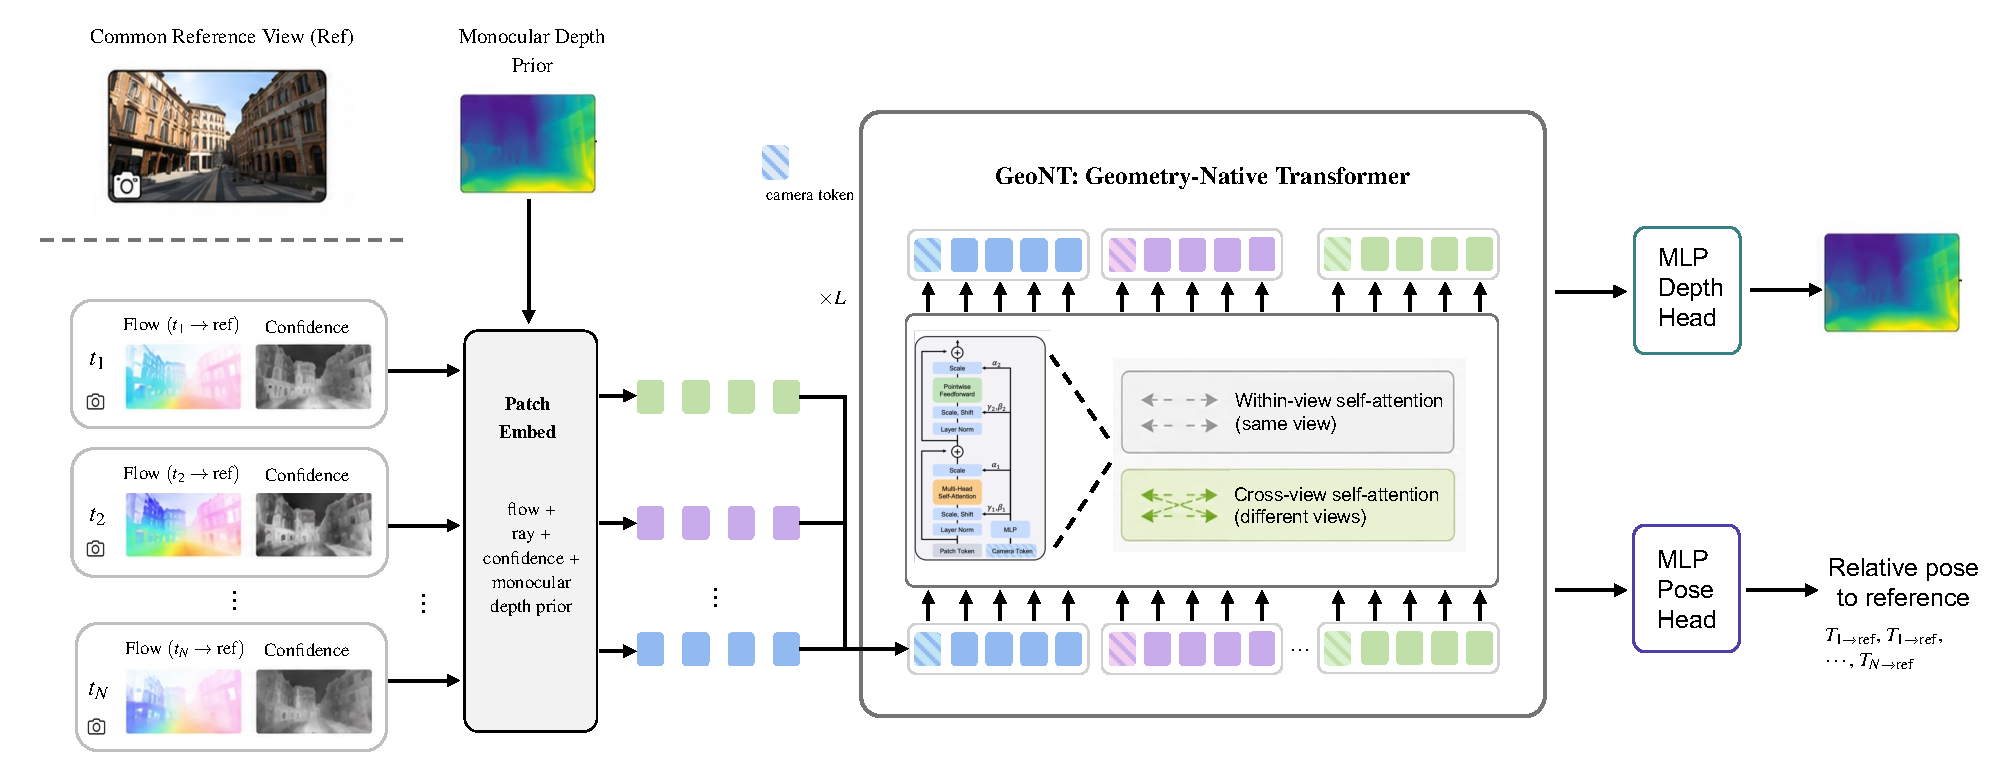
\includegraphics[width=0.99\linewidth]{fig/geont/geont.pdf}
    \vspace{-5pt}
    \caption{\textbf{Overview of the GeoNT measurement network.}
    A common reference view is paired with multiple support views.
    For each support view, reference-to-support optical flow, flow confidence, intrinsics-normalized ray information, and the normalized monocular depth prior are embedded into geometry-native patch tokens.
    A ViT-Base Geometry-Native Transformer aggregates these token fields through within-view and cross-view reasoning with camera-token conditioning, then predicts refined reference-view depth and scale-normalized relative pose measurements.
    Metric scale is handled outside the network by the pose-scale graph.}
    \label{fig:geont_overview}
    \vspace{-12pt}
\end{figure}

\subsection{From Visual Tokens to Geometry Tokens}
Geometry-native tokenization is motivated by the goal of bringing explicit correspondence into neural geometry inference.
Image-token Transformers are natural for recognition and feed-forward reconstruction, where the model must infer task-relevant structure from RGB appearance.
In a SLAM-oriented monocular video setting, however, part of the geometric evidence can be made explicit before Transformer aggregation.
Optical flow provides inter-view correspondences, flow confidence indicates their reliability, a monocular depth prior provides normalized scene-shape evidence, and camera intrinsics convert pixel grid into camera-normalized rays.
GeoNT therefore tokenizes these geometry signals directly, so the backbone reasons over quantities already tied to the rigid-projection model rather than inferring geometry from appearance alone.
This is also the main distinction from DBA-centered systems such as DROID-SLAM and MegaSaM: GeoNT does not keep a recurrent dense BA state as the primary representation.
It predicts learned depth and pose measurements from tokenized flow, uncertainty, ray, and depth-prior fields, then hands selected pose measurements to a separate graph.

This representation also serves an architectural purpose.
By exposing correspondence and depth-prior structure at the input, GeoNT shifts Transformer capacity from low-level matching toward resolving depth-motion ambiguity, multi-view consistency, and measurement confidence.
This is important for integration with streaming SLAM systems, where the network is invoked repeatedly during tracking and local mapping.
Throughout this chapter, GeoNT uses a lightweight ViT-Base backbone; the geometry-native tokens are intended to make this compact Transformer a practical aggregation module instead of relying on a larger visual-token backbone to infer geometry implicitly.

The motion token is designed to express optical flow in camera-normalized coordinates.
For a reference view $i$ and a support view $j$, a flow network predicts a dense flow field $\bm{F}_{ij}$ and a confidence field $\bm{Q}_{ij}$.
The motion tokenizer builds an intrinsics-normalized per-pixel vector
\begin{equation}
    \bm{m}_{ij}(u,v)
    =
    \left[
    \frac{u-c_x}{f_x},
    \frac{v-c_y}{f_y},
    \alpha\frac{F^x_{ij}(u,v)}{f_x},
    \alpha\frac{F^y_{ij}(u,v)}{f_y},
    q_{ij}(u,v)
    \right],
    \label{eq:geont_motion_token_input}
\end{equation}
where $(f_x,f_y,c_x,c_y)$ are the camera intrinsics, $q_{ij}$ summarizes flow confidence, and $\alpha$ is a fixed scaling factor used to keep normalized flow values numerically visible to the patch embedding.
The first two channels encode the ray direction of the pixel; the next two encode angular image motion; the final channel expresses the reliability of the flow measurement.
A patch embedding maps this field to a motion token map $\bm{M}_{ij}$.
Compared with RGB patch tokens, this representation exposes both the geometric displacement and its reliability before global aggregation begins.

The reference-depth token provides the complementary shape prior needed when temporal motion alone is ambiguous.
Let $\tilde{\bm{D}}_i$ be the normalized monocular depth prior and $\bm{M}_i^{\mathrm{valid}}$ be the valid non-sky mask.
The depth tokenizer embeds the two-channel map
\begin{equation}
    \bm{d}_i(u,v)
    =
    \left[
    \tilde{D}_i(u,v),
    M_i^{\mathrm{valid}}(u,v)
    \right].
    \label{eq:geont_depth_token_input}
\end{equation}
For a reference view with support keyframes $\mathcal{N}(i)$, the same reference-depth token map is expanded across the support-view dimension and concatenated with each motion token map:
\begin{equation}
    \bm{P}_{ij}
    =
    \operatorname{Concat}\left(\bm{D}_i^{\mathrm{tok}}, \bm{M}_{ij}\right),
    \qquad j \in \mathcal{N}(i).
    \label{eq:geont_patch_token}
\end{equation}
The resulting representation contains one geometry-token field for each relation between the reference view and a local support keyframe.
Unlike an RGB token, each token is already expressed in geometric coordinates and can be interpreted through the camera projection model.
This design gives the Transformer a direct interface to temporal geometry while still allowing learned global reasoning over the reference view and its support keyframes.

\subsection{Flow Frontend with ViT-Based Motion-Basis Initialization}
Reliable optical flow is a prerequisite for geometry-native temporal reasoning, because GeoNT treats flow as the explicit correspondence measurement from which motion tokens are built.
The challenge is that a keyframe-based mapper often compares views with a larger temporal baseline than adjacent video frames.
Local optical-flow refinement is effective when the current estimate is already close to the correct match, but it can fail when the initial field places the correlation lookup outside the correct local basin.
Wide-baseline matchers, such as RoMa~\cite{edstedt2024roma}, address a related but different operating point: they are designed to recover robust correspondences under large viewpoint changes, whereas GeoNT requires a dense, low-latency flow field whose quantities can be interpreted as camera-normalized angular motion.
In this setting, even a few pixels of localization error can be significant.
GeoNT therefore needs a frontend that combines geometry-aware wide-baseline initialization, dense subpixel refinement, and a confidence map expressed in a form suitable for Transformer aggregation.

The flow frontend is built around this two-stage correspondence design.
First, it constructs pair features by reusing the monocular depth network's encoder feature and concatenating it with a ResNet18 image feature for both the reference and support views.
The monocular feature contributes global context and scene-layout cues, while the ResNet feature preserves local texture and boundary detail for dense matching.
Second, it forms a motion-basis prior from the monocular depth prior and camera intrinsics.
For a pixel $\bm{x}=(u,v)$ in reference view $i$, let
\begin{equation}
    x_n=\frac{u-c_x}{f_x},\qquad
    y_n=\frac{v-c_y}{f_y},\qquad
    \rho_i(\bm{x})=\frac{1}{\tilde{D}_i(\bm{x})},
    \label{eq:geont_flow_ray_depth}
\end{equation}
where $(x_n,y_n)$ are camera-normalized ray coordinates and $\rho_i$ is the inverse normalized depth prior.
The frontend uses these quantities to build a set of low-dimensional flow bases~\cite{Poggi_2025_ICCV}
\begin{equation}
\begin{aligned}
    \bm{b}_{T_x} &= \rho_i[-1,0]^\top, &
    \bm{b}_{T_y} &= \rho_i[0,-1]^\top, &
    \bm{b}_{T_z} &= \rho_i[x_n,y_n]^\top, \\
    \bm{b}_{R_x}^{1} &= [0,1]^\top, &
    \bm{b}_{R_x}^{2} &= [x_ny_n,y_n^2]^\top, &
    \bm{b}_{R_y}^{1} &= [-1,0]^\top, \\
    \bm{b}_{R_y}^{2} &= [-x_n^2,-x_ny_n]^\top, &
    \bm{b}_{R_z} &= [-y_n,x_n]^\top .
\end{aligned}
\label{eq:geont_motion_basis}
\end{equation}
The translational bases are modulated by inverse depth, while the rotational bases are determined by the ray geometry.
Thus, the monocular depth prior and camera intrinsics provide a structured hypothesis space for the optical flow induced by camera motion, rather than leaving the initializer to infer large displacement from appearance alone.
This is the reason for using a motion-basis initializer in a keyframe runtime.
When a support keyframe is separated by several frames, a zero-flow or small-displacement start may make the recurrent updater search in the wrong correlation neighborhood.
The basis field gives the initializer a set of camera-motion-shaped displacement modes before local refinement begins.
It is not a generic sparse wide-baseline matcher: it produces a dense initialization in the same ray-and-depth coordinate convention used by the GeoNT tokens.

The flow frontend leverages a Transformer initializer to perform global reasoning over the projected reference-support pair feature and the embedded motion-basis feature.
To preserve optical-flow estimation efficiency, this initializer adopts a ViT-small variant.
Equivalently, the basis maps provide candidate motion modes from which a coarse initial field can be learned,
\begin{equation}
    \bm{F}_{ij}^{0}(\bm{x})
    \approx
    \sum_{k} a_{ij,k}(\bm{x})\,\bm{b}_{i,k}(\bm{x}),
    \label{eq:geont_basis_flow_init}
\end{equation}
where the coefficients are represented implicitly by the initializer rather than solved by a separate geometric optimizer.
In practice, the initializer predicts horizontal and vertical displacement-bin distributions, a convex-upsampling mask, and the hidden state used by the subsequent recurrent update.
The final dense flow is then produced by iterative correlation/update refinement, not directly by the ViT initializer:
\begin{equation}
    \bm{F}_{ij}^{r+1}
    =
    \bm{F}_{ij}^{r}
    +
    \Delta\bm{F}_{ij}^{r},
    \qquad
    \Delta\bm{F}_{ij}^{r},\bm{Q}_{ij}^{r}
    =
    \Psi\!\left(\bm{h}_{ij}^{r},
    \operatorname{Corr}_{ij}(\bm{x}+\bm{F}_{ij}^{r})\right),
    \label{eq:geont_flow_refinement}
\end{equation}
where $\bm{Q}_{ij}^{r}$ denotes the predicted confidence map.
Starting from the basis-conditioned coarse field, the refinement module samples a correlation volume around the current estimate, predicts residual flow updates, and upsamples the result to the image resolution.
Its update head also predicts information parameters, which are converted into the reliability channel used by the motion tokenizer together with intrinsics-normalized flow.
The flow frontend therefore supplies the GeoNT measurement network with dense correspondence and confidence evidence in the same camera-normalized coordinate system used by the geometry tokens.

\subsection{Geometry Patch Tokens and Camera-Token Conditioning}
Dense correspondence becomes a geometry measurement only after it is interpreted with camera context.
For a reference view $i$ and a support view $j$ in the temporal neighborhood, GeoNT observes a dense motion field and estimates how the measured pixel displacement can be explained by reference-view depth and relative camera motion.
Feed-forward geometry Transformers, such as VGGT~\cite{wang2025vggt} and DUSt3R~\cite{wang2024dust3r}, often place camera tokens and image or patch tokens in a common sequence.
This homogeneous token treatment is reasonable for offline reconstruction from a fixed set of views: all images and cameras are available simultaneously, camera information can act as an additional global cue, and self-attention can jointly update view, camera, and scene representations.
The streaming measurement problem in GeoNT is more structured.
The field $\bm{P}_{ij}$ in Equation~\ref{eq:geont_patch_token} represents spatially dense measured evidence, including flow, confidence, ray coordinates, and normalized depth, while the camera token $c_{ij}$ carries compact pair-level context for the reference-support pair.
The camera token therefore summarizes motion information from the patch tokens and controls how local pixel displacements are converted into depth and relative camera motion.
Keeping this token separate avoids treating pair-level camera context as just another spatial patch.
The same local flow vector can imply different depth or translation changes under different ray directions, intrinsics, and pair-level motion context; a compact camera token gives the network a place to maintain that global interpretation while the patch tokens preserve dense evidence.

Let $\bm{z}_{ij}^{\ell}$ denote the geometry patch tokens and $c_{ij}^{\ell}$ denote the camera token at Transformer layer $\ell$.
GeoNT prepends the camera token to the patch-token sequence so that it can aggregate pair-level motion context through attention.
At the same time, the camera token generates adaptive shift, scale, and gate parameters for the patch-token updates, in the spirit of DiT-style adaptive layer-normalization conditioning~\cite{peebles2023scalable}.
For the attention sublayer,
\begin{equation}
\begin{aligned}
    (\Delta_a,S_a,G_a) &= \phi_a\!\left(\operatorname{LN}(c_{ij}^{\ell})\right), \\
    \tilde{\bm{z}}_{ij}^{\ell} &=
    (1+S_a)\odot \operatorname{LN}(\bm{z}_{ij}^{\ell})+\Delta_a, \\
    [\bar c_{ij}^{a},\bar{\bm{z}}_{ij}^{a}]
    &= \operatorname{MSA}\!\left(
        [\operatorname{LN}(c_{ij}^{\ell}),\tilde{\bm{z}}_{ij}^{\ell}]
    \right), \\
    c_{ij}' &= c_{ij}^{\ell}+\bar c_{ij}^{a}, \qquad
    \bm{z}_{ij}' =
    \bm{z}_{ij}^{\ell}+G_a\odot\bar{\bm{z}}_{ij}^{a}.
\end{aligned}
\label{eq:geont_camera_token_attention}
\end{equation}
The MLP sublayer applies the same conditioning pattern,
\begin{equation}
\begin{aligned}
    (\Delta_m,S_m,G_m) &= \phi_m\!\left(\operatorname{LN}(c_{ij}')\right), \\
    \tilde{\bm{z}}_{ij}' &=
    (1+S_m)\odot \operatorname{LN}(\bm{z}_{ij}')+\Delta_m, \\
    [\bar c_{ij}^{m},\bar{\bm{z}}_{ij}^{m}]
    &= \operatorname{MLP}\!\left(
        [\operatorname{LN}(c_{ij}'),\tilde{\bm{z}}_{ij}']
    \right), \\
    c_{ij}^{\ell+1} &= c_{ij}'+\bar c_{ij}^{m}, \qquad
    \bm{z}_{ij}^{\ell+1} =
    \bm{z}_{ij}'+G_m\odot\bar{\bm{z}}_{ij}^{m}.
\end{aligned}
\label{eq:geont_camera_token_mlp}
\end{equation}
Here, $\operatorname{MSA}$ denotes multi-head self-attention over the concatenated camera and patch-token sequence, $\operatorname{MLP}$ denotes the token-wise feed-forward sublayer, and $\odot$ indicates channel-wise modulation broadcast over spatial patch tokens.
The layer normalizations applied to the patch-token fields, $\operatorname{LN}(\bm{z}_{ij}^{\ell})$ and $\operatorname{LN}(\bm{z}_{ij}')$, are non-affine; their shift and scale are supplied by the camera-token heads through $(\Delta_a,S_a)$ and $(\Delta_m,S_m)$.
Layer-scale and drop-path terms are omitted for readability.
The modulation heads $\phi_a$ and $\phi_m$ are zero-initialized for the shift, scale, and gate outputs, so the blocks begin close to the unconditioned backbone while allowing the camera token to learn pair-level control over patch-token processing.

This conditioning design lets the camera token progressively aggregate pair-level motion information while giving every dense geometry token access to the same camera-aware control signal.
Compared with homogeneous token mixing, it preserves the distinction between local measured geometry and compact pair-level conditioning: the camera cue modulates patch-token updates, rather than being handled as another peer token whose role is determined only through self-attention.
The design is therefore closer to adaptive conditioning than to simply adding a camera token to a larger image-token sequence.
By default, $c_{ij}$ is initialized from a learnable base embedding and acquires pair-specific meaning through attention to the motion tokens.
When an external relative-pose estimate is available, GeoNT can encode it as a small delta around this learned base token; in the current thesis, this pose-conditioned initialization is supporting infrastructure rather than the central claim.
The main claim is the separated camera-token conditioning mechanism for camera-aware geometry-token aggregation.

\subsection{Multi-View Aggregation}
Multi-view aggregation addresses the ambiguity of relying on a single temporal support view.
As shown in Figure~\ref{fig:geont_overview}, GeoNT aggregates several reference-support token fields for the same reference view.
One support keyframe may have weak parallax, another may be affected by occlusion, and a third may contain motion from dynamic objects.
Using several support keyframes gives the measurement network multiple motion observations for the same reference-depth representation.

GeoNT implements this aggregation with two attention modes.
For a reference view $i$ and support set $\mathcal{N}(i)$, the input contains one geometry-token field for each reference-support pair $(i,j)$, where $j\in\mathcal{N}(i)$.
Within-view attention applies self-attention independently inside each pair field, allowing the motion tokens, depth tokens, and camera token for $(i,j)$ to refine a local geometric explanation without mixing support views.
Cross-view, or global, attention concatenates the token fields associated with the same reference view and applies self-attention across all support pairs.
This global step lets temporal neighbors exchange evidence about the shared reference depth while preserving pair-specific motion and camera context.

The attention schedule delays global mixing until each pair has formed a local geometric representation.
The first stage applies only within-view attention, so each reference-support relation can refine its own camera-conditioned flow-depth representation before interacting with other support views.
The later stages alternate between within-view and cross-view attention: one cross-view block is inserted after every within-view block.
Overall, the schedule uses a $2{:}1$ ratio between within-view and cross-view attention, prioritizing local relation reasoning while still allowing temporal evidence exchange.
This follows the broad alternating-attention pattern used in recent feed-forward geometry Transformers such as VGGT~\cite{wang2025vggt} and DepthAnything3~\cite{lin2026depth}, while adapting it to geometry-native tokens and streaming keyframe relations.
The resulting design reduces the cost of global attention while still allowing periodic exchange of temporal evidence.
This efficiency matters in streaming inference, so GeoNT uses the ViT-Base configuration for the Geometry-Native Transformer as a compact aggregation backbone.

This design provides a structured route from pairwise geometry to temporal consensus.
Early within-view layers refine flow-depth evidence and camera-token conditioning for each support pair before expensive cross-view mixing.
Later cross-view layers compare temporal neighbors to support a shared reference-depth representation and a set of compatible relative pose measurements.
Inconsistent flow, occlusion, or independently moving objects may appear as conflicting evidence in the token representation, but GeoNT does not implement an explicit attention-time view-selection rule.
The output confidence estimates instead report the reliability of the final depth and pose measurements for graph weighting; they are not a confidence-based reweighting mechanism inside Transformer aggregation.

\subsection{Depth, Pose, and Confidence Heads}
The output heads in GeoNT convert the shared geometry representation into compact depth and pose measurements.
This design follows from the representation: by the end of the Geometry-Native Transformer, the tokens already encode camera-conditioned temporal geometry across the local support set.
The heads therefore read out the required measurements from the final geometry representation rather than performing heavy visual reconstruction.
This differs from visual feature Transformers, where the decoder often must fuse multi-scale appearance features before dense geometry can be recovered.

GeoNT uses several confidence-like quantities with different semantics.
The flow confidence $q_{ij}$ is an input-side correspondence reliability produced by the frontend and embedded into the motion tokens.
The depth-observability score $g_d$ is an internal support-view gate used only to fuse pairwise token fields for depth prediction.
The output depth confidence $\hat{\bm{C}}_i$ is a dense reliability estimate attached to the predicted reference-view depth.
The pose head predicts translation and rotation confidence for each directed pair; in the pose-scale graph, these values are interpreted as learned uncertainty, or equivalently as diagonal inverse-variance information, for measurement weighting.
These quantities are not interchangeable, and a high value in one does not automatically imply a high value in the others.

The depth head converts the temporally aggregated geometry representation into a dense refined depth map and a dense confidence map for the reference view.
It reads the final multi-view geometry-token representation produced by the aggregation backbone.
For a reference view $i$ and each support keyframe $j\in\mathcal{N}(i)$, this representation contains a camera-conditioned patch-token field $\bm{z}_{ij}^{\star}$ that encodes confidence estimates and depth evidence for that pair.
Before dense prediction, GeoNT integrates the depth evidence from multiple support keyframes into a coherent reference-view depth representation through learned gate-based aggregation.
Let $H\times W$ denote the reference-view resolution and $\bm{p}$ index a location on the $H/16\times W/16$ ViT patch grid.
The aggregation produces a single reference-view geometry field $\bar{\bm{z}}_i$ on this patch grid:
\begin{equation}
    \bar{\bm{z}}_i(\bm{p})
    =
    \sum_{j\in\mathcal{N}(i)}
    \alpha_{ij}(\bm{p})\,\bm{z}_{ij}^{\star}(\bm{p}),
\label{eq:geont_depth_view_aggregation}
\end{equation}
where $\alpha_{ij}(\bm{p})=\operatorname{softmax}_{j\in\mathcal{N}(i)} g_d(\bm{z}_{ij}^{\star})(\bm{p})$, and $g_d$ predicts an internal depth-observability score for each reference-support pair.
This observability weight is distinct from the output depth confidence: it determines how strongly each support keyframe contributes to the fused depth representation, so pairs with weak depth cues, such as near-pure rotation or very small parallax, can be assigned lower influence.
The compact field $\bar{\bm{z}}_i$ is then decoded by a two-stage coarse-to-dense token readout:
\begin{equation}
\begin{aligned}
    \bm{\phi}_i
    &=
    \mathcal{F}_d\!\left(
        \mathcal{U}_2(\bar{\bm{z}}_i),
        \mathcal{E}_8(\tilde{\bm{D}}_i,\bm{M}_i^{\mathrm{valid}})
    \right),\\
    [\hat{\bm{D}}_i,\hat{\bm{C}}_i]
    &=
    \mathcal{R}_8\!\left(h_d(\bm{\phi}_i)\right).
\end{aligned}
    \label{eq:geont_depth_dense_readout}
\end{equation}
Here, $\mathcal{U}_2$ denotes a learned projection followed by a pixel shuffle operation, which rearranges channel groups from each $1/16$-scale token into a $2\times2$ neighborhood on the $H/8\times W/8$ geometry feature map.
In parallel, $\mathcal{E}_8$ embeds the normalized depth prior and its validity cue with stride $8$, producing a residual prior feature on the same $H/8\times W/8$ grid.
The fusion module $\mathcal{F}_d$ combines these two features channel-wise and applies a lightweight Transformer/MLP-style readout on the $1/8$ grid, yielding the fused representation $\bm{\phi}_i$.
The final predictor $h_d$ outputs depth and confidence values for the $8\times8$ image block associated with each $1/8$-scale grid cell, and the pixel shuffle operation $\mathcal{R}_8$ rearranges these per-block predictions to restore the dense maps $\hat{\bm{D}}_i$ and $\hat{\bm{C}}_i$ at the preprocessed reference-view resolution $H\times W$.
This makes the token-to-image recovery explicit: temporal depth evidence is carried by the aggregated geometry tokens, while local scene-shape detail that may be weakened by patch-level compression is reintroduced through the residual normalized-depth branch.
Because the geometry-native aggregation backbone has already exchanged temporal evidence across support keyframes, dense recovery can remain lightweight and does not require a heavy DPT-style multi-layer visual fusion decoder~\cite{ranftl2021vision} in the default GeoNT design.

The pose head reads motion measurements from the compact camera tokens.
For each reference-support pair, the final camera token provides a pair-level representation that feeds a lightweight pose decoder for relative translation, quaternion rotation, and translation/rotation confidence.
The pose confidence values express the reliability of the final neural pose measurements for graph optimization; they are uncertainty estimates, not a mechanism for reweighting views inside multi-view attention.
Thus, the heads are deliberately compact: they expose refined depth, pose, and confidence from the shared GeoNT representation, while the central contribution remains the geometry-native Transformer representation and camera-conditioned aggregation.

\subsection{Training the GeoNT Measurement Network}
GeoNT is trained to produce temporal geometry measurements that can be used by a streaming local map.
The supervision must couple scene shape with camera motion: a depth estimate is useful only if, together with the predicted relative pose, it explains the observed correspondence between views.
Accordingly, training asks GeoNT to predict three kinds of measurements for a reference view and its support views: a refined normalized depth map, relative poses whose translation magnitude is expressed in the reference view's normalized depth scale, and reliability estimates for the depth and pose outputs.
The flow frontend is trained in the same measurement setting, because its correspondence estimates are the motion evidence from which the geometry tokens are formed.

Training samples are constructed from video sequences with ground-truth camera poses, depth maps, and intrinsics.
Following the frame-graph training practice of DROID-SLAM~\cite{teed2021droid}, supervision is organized by a graph over geometrically connected frames rather than by adjacent frame pairs alone.
Frames and graph edges are selected using geometric covisibility measured by induced optical-flow distance, so useful training pairs have both sufficient overlap and meaningful image motion.
Each directed graph edge defines a reference-support pair for GeoNT, and the outgoing edges of a reference frame provide the support set used for multi-view aggregation.
This construction matches the intended measurement setting: GeoNT learns from video frames that are connected by observable geometry, not from unordered image sets or from a fixed temporal spacing.

During training, the forward path follows the measurement network described above.
The monocular geometry model provides a normalized depth prior for each frame.
The flow frontend predicts dense flow and flow reliability on the sampled graph edges; these quantities are embedded with camera-normalized ray coordinates to form geometry patch tokens.
The Geometry-Native Transformer processes the reference-support token fields with separate camera tokens and outputs refined normalized depth, relative pose measurements, depth reliability maps, and pose reliability values.
For a graph edge from reference view $i$ to support view $j$, the translation target is compared in the normalized depth scale of view $i$, while rotation is supervised through the quaternion representation.
This convention keeps pose supervision compatible with the normalized-depth representation used by the GeoNT measurement system.

The training objective is a compact multi-task loss,
\begin{equation}
    \mathcal{L}_{\mathrm{train}}
    =
    \lambda_{\mathrm{depth}} \mathcal{L}_{\mathrm{depth}}
    +
    \lambda_{\mathrm{pose}} \mathcal{L}_{\mathrm{pose}}
    +
    \lambda_{\mathrm{proj}} \mathcal{L}_{\mathrm{proj}}
    +
    \lambda_{\mathrm{flow}} \mathcal{L}_{\mathrm{flow}},
    \label{eq:geont_training_objective}
\end{equation}
where the weights balance depth, pose, projective geometry, and optical-flow supervision.
The depth loss applies the same valid-mask normalization to predicted and ground-truth depth before comparison, so the depth head is supervised in the normalized gauge used by the runtime; multi-scale depth-gradient terms preserve local shape.
The pose loss compares directed relative poses on graph edges: translation is evaluated after division by the reference keyframe's depth scale, and rotation is evaluated by the quaternion or Lie-algebra residual used by the pose head.
The projective consistency loss checks the joint measurement by encouraging predicted normalized depth and predicted relative pose to induce correspondences consistent with ground-truth depth, pose, and intrinsics under the rigid projection model.
The flow loss supervises both the ViT-based initializer and the recurrent refinement using projective flow targets, because flow is the explicit correspondence evidence from which the geometry tokens are formed.
Reliability weighting follows a heteroscedastic uncertainty interpretation: residuals are downweighted by predicted uncertainty or upweighted by predicted inverse variance, while the corresponding log-uncertainty regularizer discourages the trivial solution of declaring all measurements unreliable.

Frame-graph supervision and projective geometric losses provide the training structure for these feed-forward measurement readouts~\cite{teed2021droid}.
The trained outputs are refined reference depth, relative pose in the reference depth scale, and reliability estimates that can be used by the streaming pose-scale graph.
The next section explains how these measurements become transient tracking estimates, keyframe-aligned depth, and graph constraints in the streaming runtime.

\section{Streaming Local Mapping Runtime}
\label{sec:geont_streaming}

\begin{figure}[!t]
    \centering
    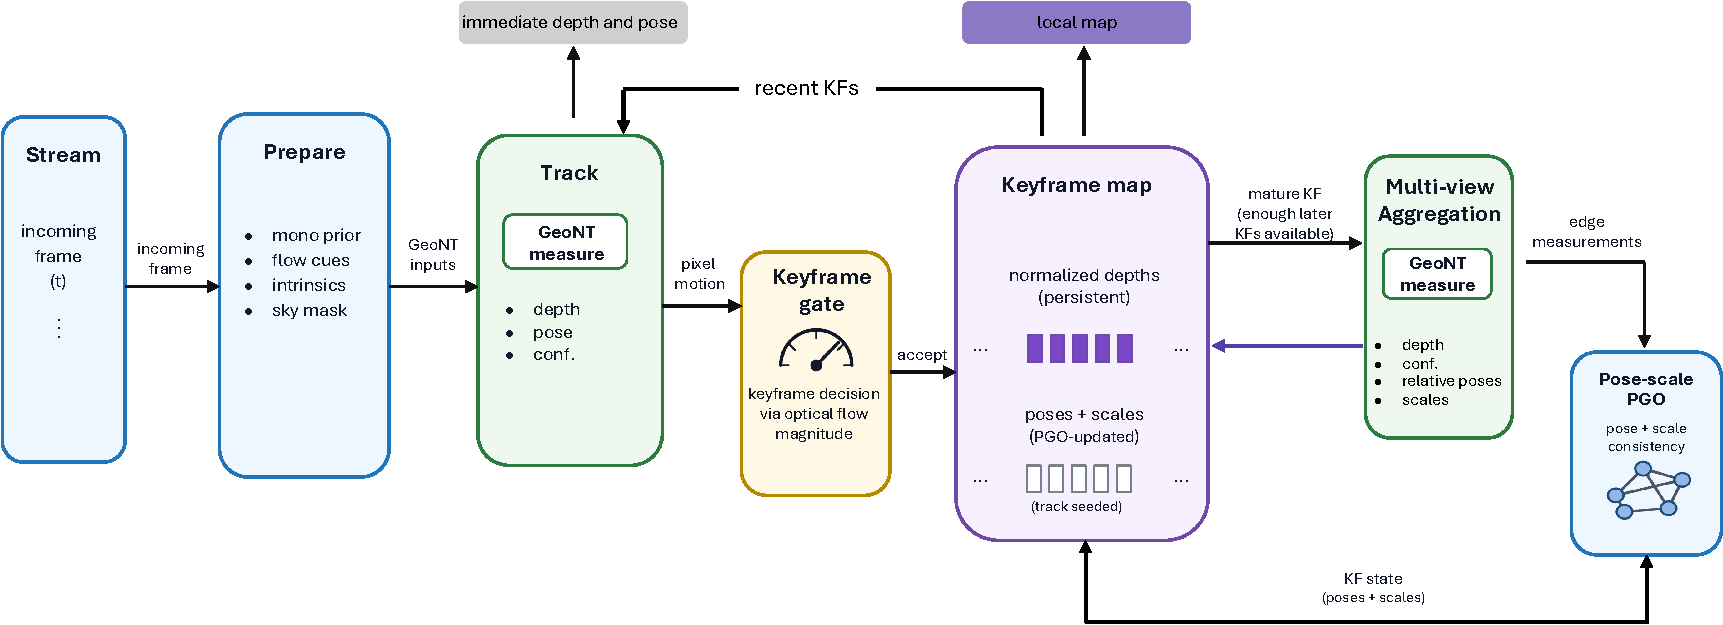
\includegraphics[width=0.99\linewidth]{fig/geont/runtime.pdf}
    \vspace{-5pt}
    \caption{\textbf{Overview of the GeoNT streaming local mapping runtime.}
    Incoming frames first support low-latency tracking inference for immediate depth and motion.
    Selected frames become keyframe nodes in the active local map.
    A selected keyframe receives temporal refinement after sufficient neighboring support keyframes are available, allowing GeoNT to compute one consolidated multi-view depth estimate.
    Pose-scale optimization then smooths keyframe motion and metric depth scale while dense geometry remains attached to keyframes.}
    \label{fig:geont_runtime}
    \vspace{-10pt}
\end{figure}

\subsection{Runtime Overview}
GeoNT is deployed as a keyframe-based streaming mapper rather than an offline sequence processor.
Figure~\ref{fig:geont_runtime} illustrates how incoming frames become immediate tracking estimates, keyframe-aligned local geometry, pose-scale graph constraints, and a recovered frame-level trajectory.
The runtime is organized around a mapping contract.
For each incoming frame, GeoNT can provide immediate depth and relative motion with respect to recent keyframes, which supports low-latency response before any keyframe mapping decision is made.
Only selected frames become keyframes, and dense geometry is maintained only at keyframes in the active local map.
After sufficient temporal support becomes available, each selected keyframe receives a single multi-view depth consolidation.
Pose graph optimization then adjusts keyframe pose and metric scale, but it does not change the normalized keyframe depth map.
Table~\ref{tab:geont_runtime_stages} summarizes this separation between online response, keyframe-aligned dense geometry, and graph-level scale adjustment.
Figure~\ref{fig:geont_active_local_map} illustrates the dense geometry maintained in the active local map around the current keyframe.

\begin{table}[!t]
    \centering
    \caption{\textbf{Runtime stages for GeoNT streaming local mapping.}
    The table summarizes how online tracking, keyframe depth estimation, and pose-scale optimization remain separated.}
    \label{tab:geont_runtime_stages}
    \small
    \setlength{\tabcolsep}{4pt}
    \renewcommand{\arraystretch}{1.12}
    \begin{tabular*}{\textwidth}{@{\extracolsep{\fill}}p{0.18\textwidth}p{0.33\textwidth}p{0.39\textwidth}@{}}
        \toprule
        \textbf{Mapping stage} & \textbf{Estimation role} & \textbf{State or measurement} \\
        \midrule
        Frame geometry inputs &
        Measurement evidence for GeoNT &
        Each frame is represented by fixed intrinsics, a normalized monocular depth prior, a validity cue, and flow-based correspondence evidence. \\
        Support selection &
        Local temporal context with useful parallax and overlap &
        Low-latency tracking uses nearby keyframes; backend refinement uses a local temporal neighborhood; optional retrieval contributes pose-only graph support. \\
        Frontend tracking &
        Immediate geometric response before keyframe admission &
        Transient depth, depth confidence, and relative motion support immediate response; dense geometry is maintained only for selected keyframes in the active local map. \\
        Keyframe admission &
        Keyframe-aligned local geometry &
        Keyframe admission selects reliable geometric novelty using cues such as flow or pose magnitude, temporal spacing, overlap, tracking validity, and confidence; admitted frames become the keyframe nodes whose dense geometry is later refined with temporal support. \\
        Backend temporal refinement &
        Consolidated keyframe depth after temporal support becomes available &
        Each selected keyframe receives one temporally refined normalized depth estimate after sufficient neighboring support keyframes are available; graph optimization later changes only pose and scale. \\
        Pose-edge formation &
        Graph-compatible motion constraints &
        Temporal and optional proximity measurements provide reference-scale-normalized pose constraints with confidence weights; these constraints do not modify dense geometry. \\
        Pose-scale optimization &
        Local pose-scale consistency &
        PGO optimizes keyframe poses and node scales under the GeoNT edge convention while keeping all keyframe depth maps fixed. \\
        Final mapping state &
        Local map and trajectory estimate &
        The final mapping state consists of keyframe poses, keyframe depths, optimized scales, edge statistics, and a recovered full-frame trajectory. \\
        \bottomrule
    \end{tabular*}
\end{table}

\begin{figure}[!t]
    \centering
    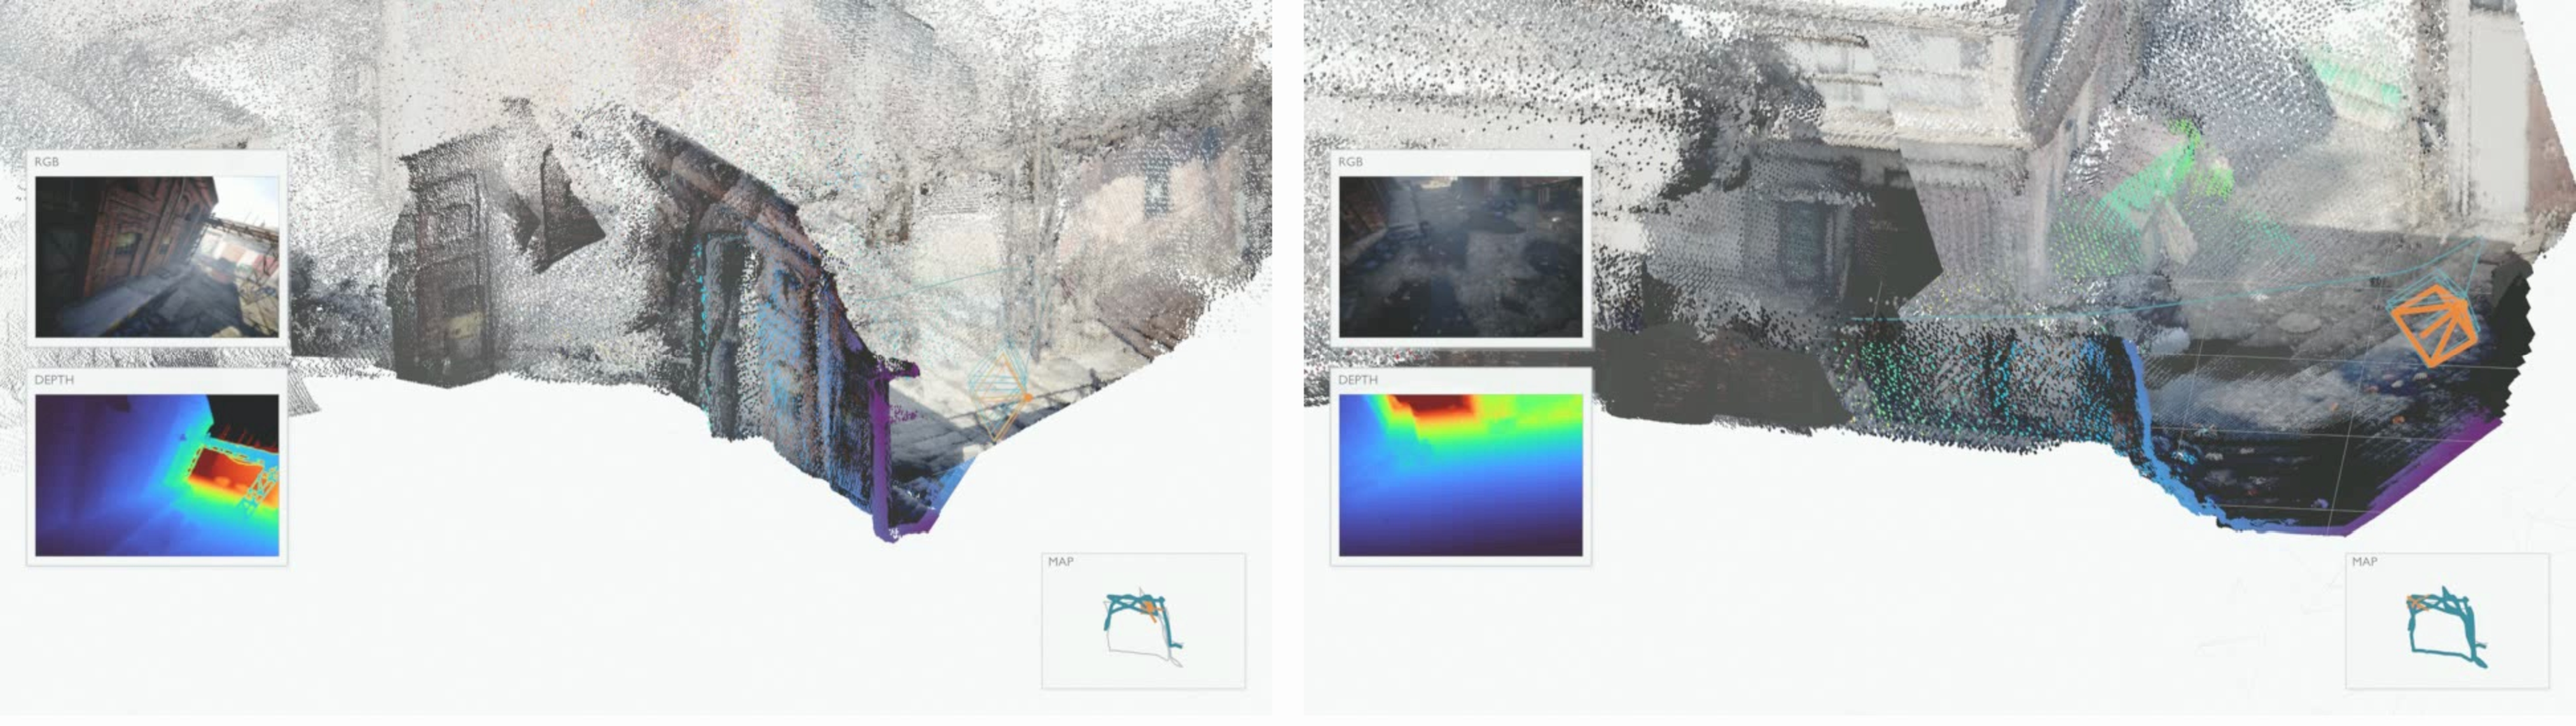
\includegraphics[width=0.99\linewidth]{fig/geont/local_map_twopanel.pdf}
    \caption{\textbf{Active local map in GeoNT.}
    The visualization shows the current keyframe together with its reconstructed dense local geometry.
    It illustrates the keyframe-aligned mapping output produced after temporal multi-view aggregation, rather than the sparse pose-scale graph used for optimization.
    This view emphasizes the dense geometric state that GeoNT contributes to the active local map.}
    \label{fig:geont_active_local_map}
\end{figure}

\subsection{Frontend Tracking and Keyframe Admission}
Frontend tracking is the low-latency stage that provides immediate depth and pose estimates for each incoming frame.
The first frame initializes the local map with its monocular depth prior.
For later frames, GeoNT tracking aggregation relates the current frame to recent $K$ keyframes, producing refined depth and relative poses.
The tracking evidence also supports keyframe admission as a secondary decision: optical-flow magnitude and tracking validity indicate whether the current frame adds a reliable and distinct geometric view.
Frames that are not selected as keyframes keep their estimates as transient tracking quantities for low-latency robotic response; dense geometry remains keyframe-aligned in the active local map.
Their relative poses still provide the frame-to-keyframe relations needed to reconstruct the full-frame trajectory after keyframe optimization.
Keyframe admission only decides whether an incoming frame should become part of the active local map; it does not make the transient tracking depth the final keyframe geometry.
When a frame is selected as a keyframe, its pose is initialized from the relative motion to the previous keyframe, while its keyframe-aligned dense geometry is established later through temporal multi-view refinement after sufficient support keyframes are available.

In this way, tracking remains an immediate-response mechanism, whereas keyframe-aligned normalized depth and graph factors come from multi-view aggregation of covisible supported keyframes.
Non-keyframe poses are preserved without turning every frame into a graph node.
Each non-keyframe keeps its online relative pose to a reference keyframe.
After the final graph optimization, the full-frame trajectory is recovered from these relative motion estimates, the optimized reference keyframe poses, and the reference keyframe scale corrections.
The result is a compact keyframe graph together with a full-frame trajectory, while dense mapping remains keyframe-based and non-keyframe depth stays transient.

\subsection{Backend Temporal Refinement}
Backend temporal refinement improves a selected keyframe after sufficient temporal support becomes available.
The frontend depth estimate serves low-latency response, but it may initially rely on only one or two recent neighbors.
The local mapping radius $r$ defines when a keyframe has sufficient temporal support for consolidation.
Keyframe $i$ is refined once the active keyframe sequence includes keyframe $i+r$, so that its temporal support set contains the neighboring views needed for multi-view aggregation.
GeoNT then aggregates reference keyframe $i$ with its temporal support set once, producing the consolidated keyframe-aligned depth map $\bm{D}_i$.
The keyframe scale is updated by matching the mean normalized depth before and after this multi-view refinement:
\begin{equation}
    s_i \leftarrow
    s_i
    \frac{
        \operatorname{mean}_{\bm{x}\in\Omega_i}\tilde{D}_i(\bm{x})
    }{
        \operatorname{mean}_{\bm{x}\in\Omega_i}D_i(\bm{x})
    },
    \label{eq:geont_temporal_scale_update}
\end{equation}
where $\Omega_i$ denotes valid non-sky pixels.
This update keeps the keyframe's average valid depth scale aligned with the original monocular gauge while allowing temporal refinement to change local structure.
The resulting scale becomes the keyframe's node-scale estimate before graph optimization.

Temporal refinement also determines which GeoNT measurements enter the pose graph.
During the multi-view aggregation that consolidates a keyframe depth estimate, GeoNT predicts keyframe-relative poses to its support keyframes together with reliability weights.
Each directed keyframe relation is represented as one weighted pose-graph factor.
This schedule keeps the local map interpretable: each keyframe receives one multi-view consolidated dense estimate, and each GeoNT relative-pose measurement becomes a graph factor only after the supporting temporal neighborhood has been observed.

\subsection{Depth Lifecycle and Metric Interpretation}
The mapping formulation separates the monocular depth prior, the keyframe-aligned depth map, and the optimized metric scale.
The normalized monocular prior $\tilde{\bm{D}}_i$ is the depth input to GeoNT and is not replaced by later keyframe estimates.
The keyframe-aligned depth map $\bm{D}_i$ represents the normalized scene shape associated with keyframe $i$ in the active local map.
For keyframes with sufficient temporal support, backend multi-view aggregation consolidates this representation across neighboring views.
The node scale $s_i$ is the graph-optimized scalar that gives this normalized depth representation its metric interpretation through Equation~\ref{eq:geont_metric_depth}.

Frontend tracking provides transient depth for immediate response, while backend temporal refinement establishes the temporally consolidated keyframe estimate.
PGO may later update $s_i$, but it does not rewrite $\bm{D}_i$.
When the optimized scale changes, the metric interpretation of the keyframe depth changes through $\bm{Z}_i=s_i\bm{D}_i$.
Thus, the active local map exposes keyframe depth together with the current scale needed to use that depth metrically.
Dense geometry is therefore keyframe-aligned, while transient non-keyframe depth remains available for online response without becoming part of the maintained local map state.

\section{Pose Graph Optimization}
\label{sec:geont_pgo}

\subsection{Graph State and Residuals}
Pose graph optimization is a consistency layer over GeoNT measurements, not the dense reconstruction engine of the system.
The graph optimizes keyframe poses and node scales while leaving the keyframe normalized depth maps fixed.
Let $\bm{T}_i \in SE(3)$ be the pose of keyframe $i$, and let $\ell_i=\log s_i$ be its log scale.
For each directed edge $(i,j)$, GeoNT provides a measured relative pose $(\hat{\bm{t}}_{ij},\hat{\bm{R}}_{ij})$ and confidence weights.
The translation residual follows the reference-scale-normalized convention:
\begin{equation}
    \bm{r}^{t}_{ij}
    =
    \frac{\operatorname{trans}(\bm{T}_j\bm{T}_i^{-1})}{\exp(\ell_i)}
    -
    \hat{\bm{t}}_{ij}.
    \label{eq:geont_translation_residual}
\end{equation}
The rotation residual is
\begin{equation}
    \bm{r}^{R}_{ij}
    =
    \log\!\left(
        \hat{\bm{R}}_{ij}^{-1}
        \bm{R}_j
        \bm{R}_i^{-1}
    \right),
    \label{eq:geont_rotation_residual}
\end{equation}
where $\log(\cdot)$ maps from $SO(3)$ to its Lie algebra.
A soft node-scale prior keeps optimized scales near the pre-optimization keyframe scales:
\begin{equation}
    r^s_i = \ell_i - \ell_i^0 .
    \label{eq:geont_scale_prior}
\end{equation}
The prior strength is controlled by a scalar scale-confidence parameter.

The full objective is
\begin{equation}
    \min_{\{\bm{T}_i,\ell_i\}}
    \sum_{(i,j)\in\mathcal{E}}
    \rho\!\left(
        \left\|
        \bm{W}_{ij}
        \begin{bmatrix}
        \bm{r}^{t}_{ij}\\
        \bm{r}^{R}_{ij}
        \end{bmatrix}
        \right\|_2^2
    \right)
    +
    \lambda_s
    \sum_i
    \left(r_i^s\right)^2,
    \label{eq:geont_pgo_objective}
\end{equation}
where $\bm{W}_{ij}$ is built from GeoNT translation and rotation confidence, $\rho$ is a robust penalty, and $\lambda_s$ is the scale-prior strength.
The anchor pose is fixed by excluding its pose delta from optimization.
The anchor scale remains optimized under the soft scale prior.
This objective uses neural relative-pose measurements as soft constraints and uses pose confidence to decide how strongly each inserted edge should influence the graph.
The graph weight $\bm{W}_{ij}$ is an edge-level diagonal information matrix derived from the pose head's learned translation and rotation uncertainty, together with fixed graph-level scaling choices and the robust penalty.
It does not introduce dense photometric or geometric residuals over all pixels.

\subsection{Joint SE(3)-Scale Optimization}
The pose-scale graph is optimized jointly because GeoNT translation measurements are expressed in the normalized depth gauge of the reference keyframe.
A change in the node scale therefore changes the metric interpretation of both the keyframe depth map and the outgoing translation residuals.
The graph consequently estimates the $SE(3)$ keyframe poses and the log-scales $\ell_i$ in a single objective, balancing reference-scale-normalized pose residuals against the soft node-scale prior in Equation~\ref{eq:geont_pgo_objective}.
This joint formulation smooths local motion and metric scale while leaving the keyframe-aligned normalized depth maps fixed.
PGO is therefore a consistency layer over GeoNT relative-pose measurements and keyframe scales, rather than a late dense reconstruction stage.

\section{Evaluation Protocol and Analysis}
\label{sec:geont_eval_protocol}

\subsection{Local Mapping Evaluation Scope}
Since GeoNT is designed as a local mapping module, the evaluation is organized around the quantities that make the active local map geometrically useful: keyframe-aligned depth for local dense structure and pose-graph factors for pose-scale consistency.
The first question is whether temporal multi-view aggregation improves the depth maps associated with selected keyframes relative to the monocular prior.
The second question is whether the GeoNT relative-pose measurements that become pose-graph factors are geometrically reliable, with translation evaluated after alignment to the ground-truth metric scale.
This scope matches the present experimental stage: the chapter evaluates keyframe depth under a consistent video-level scale and measures GeoNT relative-pose factors directly.

\subsection{Keyframe Depth Evaluation}
Depth evaluation compares keyframe-aligned depth maps against ground-truth depth on selected keyframes.
Because monocular depth is scale ambiguous, each video sequence is evaluated with a single alignment scale shared by all evaluated keyframes in that video.
Let $\mathcal{K}_v$ denote the selected keyframes in video $v$ and let $\alpha_v$ denote the video-level alignment scale computed over the union of valid pixels from these keyframes.
All predicted keyframe depths in the video are evaluated as $\alpha_v \bm{D}_i$ for $i\in\mathcal{K}_v$.
The scale is not re-estimated separately for each keyframe, so the protocol evaluates keyframe depth quality under a consistent sequence-level gauge.

The reported metrics are the standard depth errors, including AbsRel, RMSE, RMSE-log, and $\delta$ accuracy thresholds.
The depth comparison includes the MoGe2~\cite{wang2025moge2} monocular prior, DROID-SLAM~\cite{teed2021droid}, DepthAnything3~\cite{lin2026depth} in sliding-window mode, and the GeoNT keyframe-aligned depth after backend multi-view aggregation.
These baselines separate the empirical roles of single-view depth prior, dense BA-centered SLAM depth, and feed-forward multi-view geometry in a chunked sliding-window setting.
The DepthAnything3 setting is therefore not a strict low-latency streaming system; it provides a strong feed-forward geometry reference although operating with substantial window-level latency.

\begin{table}[!t]
    \centering
    \caption{\textbf{Keyframe depth evaluation on TartanAir.}
    Metrics are averaged over 32 sequences.
    GeoNT is evaluated using the keyframe-aligned depth after backend multi-view aggregation.}
    \label{tab:geont_depth_eval}
    \small
    \setlength{\tabcolsep}{5pt}
    \renewcommand{\arraystretch}{1.12}
    \begin{tabular*}{\textwidth}{@{\extracolsep{\fill}}lcccccc@{}}
        \toprule
        \textbf{Method} &
        \textbf{AbsRel}$\downarrow$ &
        \textbf{RMSE}$\downarrow$ &
        \textbf{RMSE$_{\log}$}$\downarrow$ &
        \textbf{$\delta_1$}$\uparrow$ &
        \textbf{$\delta_2$}$\uparrow$ &
        \textbf{$\delta_3$}$\uparrow$ \\
        \midrule
        MoGe2 prior~\cite{wang2025moge2} & 0.084 & 2.798 & 0.169 & 0.914 & 0.965 & 0.980 \\
        DROID-SLAM~\cite{teed2021droid} & 0.414 & 34.080 & 0.324 & 0.854 & 0.917 & 0.947 \\
        DepthAnything3 (sliding-window)~\cite{lin2026depth} & 0.073 & 2.804 & 0.151 & \textbf{0.936} & 0.970 & 0.982 \\
        GeoNT (ours) & \textbf{0.066} & \textbf{2.503} & \textbf{0.142} & 0.936 & \textbf{0.971} & \textbf{0.984} \\
        \bottomrule
    \end{tabular*}
\end{table}

Table~\ref{tab:geont_depth_eval} shows that GeoNT improves the keyframe-aligned depth over the monocular prior and over the chunked feed-forward baseline on the main error metrics.
The DROID-SLAM row provides concrete evidence for the chapter motivation: although dense BA is effective for pose estimation, its depth errors are substantially larger in this protocol, with AbsRel increasing from 0.066 for GeoNT to 0.414 and RMSE increasing from 2.503 to 34.080.
This gap is especially visible in distant or weakly textured regions, where photometric BA has limited depth leverage and tends to produce less reliable dense geometry.
Overall, the result supports the local-mapping motivation: temporal support can improve the dense geometry attached to selected keyframes, while graph-compatible pose measurements are evaluated separately in the next subsection.

\subsection{Graph Factor Evaluation}
Graph factor evaluation measures GeoNT relative-pose measurements directly in the graph domain.
For each directed keyframe factor $(i,j)$, the predicted relative rotation is compared with the ground-truth relative rotation by geodesic rotation error.
The predicted translation is produced in the reference-scale-normalized convention used by the graph, so the translation vector is scale-aligned to the corresponding ground-truth relative translation before computing its metric error.
For each directed factor $(i,j)$, let $\bm{t}^{\mathrm{gt}}_{ij}=\operatorname{trans}(\bm{T}^{\mathrm{gt}}_j(\bm{T}^{\mathrm{gt}}_i)^{-1})$.
The per-factor alignment scale is
\begin{equation}
    \beta_{ij}
    =
    \arg\min_{\beta>0}
    \left\|
        \beta \hat{\bm{t}}_{ij} - \bm{t}^{\mathrm{gt}}_{ij}
    \right\|_2^2 .
    \label{eq:geont_factor_scale_alignment}
\end{equation}
Translation error is then measured between $\beta_{ij}\hat{\bm{t}}_{ij}$ and $\bm{t}^{\mathrm{gt}}_{ij}$, while translation direction error is evaluated directly because it is scale invariant.
This protocol asks whether each GeoNT factor provides a geometrically meaningful local motion constraint after the per-edge monocular scale ambiguity has been removed.

\begin{table}[!t]
    \centering
    \caption{\textbf{GeoNT graph-factor evaluation on TartanAir.}
    Metrics are computed over 73,919 directed keyframe factors from 32 sequences.
    Translation error is computed after directly aligning each factor translation to its ground-truth relative translation using Equation~\ref{eq:geont_factor_scale_alignment}.}
    \label{tab:geont_factor_eval}
    \small
    \setlength{\tabcolsep}{6pt}
    \renewcommand{\arraystretch}{1.12}
    \begin{tabular*}{\textwidth}{@{\extracolsep{\fill}}lccc@{}}
        \toprule
        \textbf{Metric} & \textbf{Mean} & \textbf{Median} & \textbf{90th pct.} \\
        \midrule
        Rotation error (deg)$\downarrow$ & 0.098 & 0.074 & 0.202 \\
        Translation direction error (deg)$\downarrow$ & 1.315 & 0.732 & 2.497 \\
        Scale-aligned translation error (m)$\downarrow$ & 0.015 & 0.008 & 0.032 \\
        \bottomrule
    \end{tabular*}
\end{table}

Table~\ref{tab:geont_factor_eval} shows that the GeoNT factors provide accurate relative rotations and translation directions, which are the two most directly scale-invariant parts of the learned motion measurement.
The translation confidence also behaves as a useful reliability signal for graph optimization: factors in the highest confidence quartile have a mean scale-aligned translation error of 0.006, compared with 0.026 for the lowest confidence quartile.
This confidence-error relation supports using learned factor weights in the pose-scale graph, while keeping the evaluation centered on local GeoNT measurement.

Figure~\ref{fig:geont_odometry_trajectory} visualizes the cumulative behavior obtained by integrating the local relative-pose estimates over one representative sequence.
The estimated trajectory follows the ground-truth path after Sim(3) alignment, showing that the local factors provide usable odometry constraints.
At the same time, the remaining deviation reflects the expected limitation of pure odometry: without loop closure, local pose errors and scale drift can accumulate over long trajectories.

\begin{figure}[!t]
    \centering
    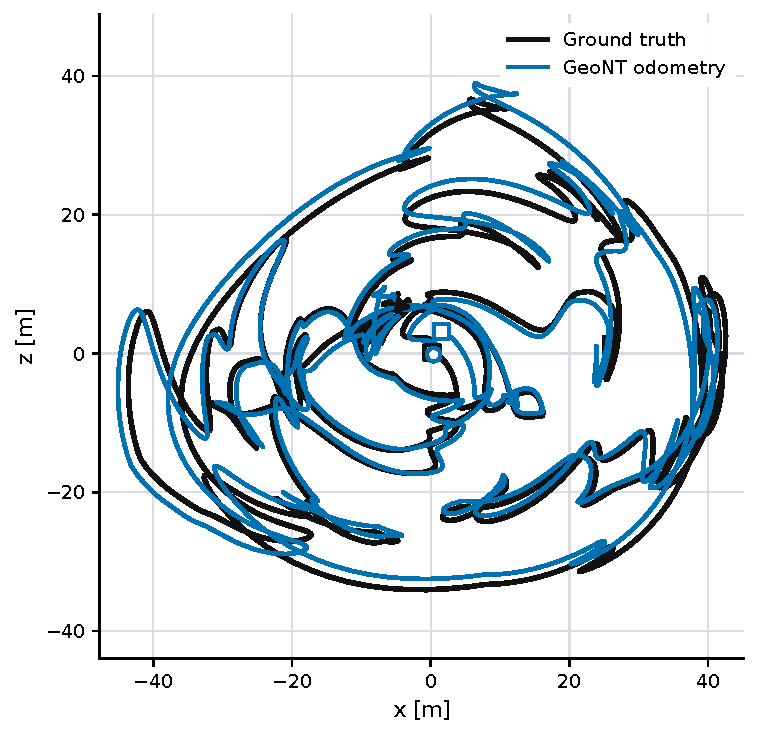
\includegraphics[width=0.76\linewidth]{fig/geont/odometry_trajectory_p011.pdf}
    \caption{\textbf{Odometry trajectory from GeoNT relative-pose integration.}
    The plot compares the GeoNT odometry trajectory with ground truth on the TartanAir abandonedfactory/Easy/P011 sequence.
    The trajectory is Sim(3)-aligned for visualization and is obtained by integrating local relative-pose estimates without loop closure.
    The result illustrates pose-estimation consistency at the odometry level, while the residual drift motivates loop closure or long-range constraints for global trajectory correction.}
    \label{fig:geont_odometry_trajectory}
\end{figure}

\begin{figure}[!t]
    \centering
    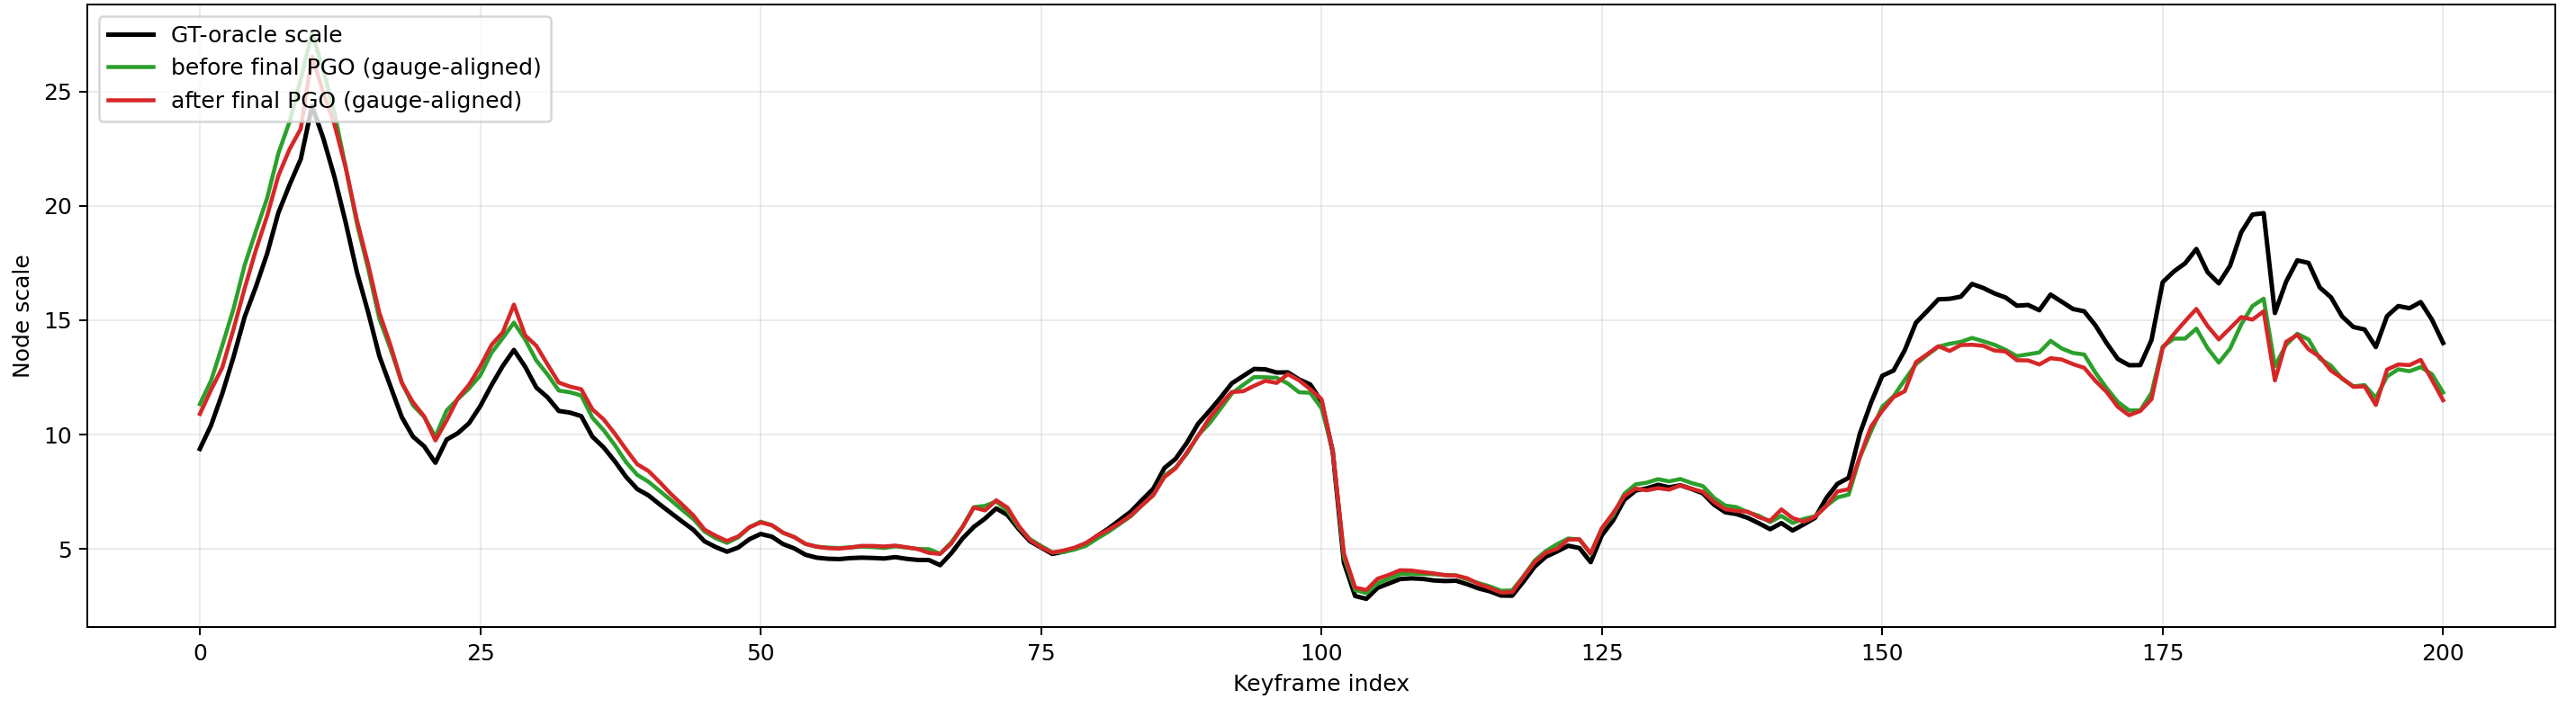
\includegraphics[width=\textwidth]{fig/geont/scale_factor_visualization.png}
    \caption{\textbf{Scale-factor behavior in a representative TartanAir sequence.}
    The black curve shows the oracle keyframe scale obtained from ground-truth depth, while the green and red curves show the gauge-aligned node scales before and after final pose-scale optimization.
    The estimated scales preserve the local relative scale trend, but a long-range scale drift remains because the current graph is built from local temporal constraints rather than loop-closure constraints.}
    \label{fig:geont_scale_factor_visualization}
\end{figure}

Figure~\ref{fig:geont_scale_factor_visualization} illustrates the role and limitation of the pose-scale graph.
The estimated scale curves follow the local variations of the oracle scale, indicating that GeoNT factors provide locally consistent scale information for nearby keyframes.
However, the curves gradually deviate from the oracle scale over the longer sequence, especially in later portions where local constraints cannot anchor the accumulated gauge drift.
This behavior is expected for a local mapping formulation: PGO smooths pose and scale over the active graph, but without loop closure or long-range scale anchors it cannot fully correct global scale drift.
Adding loop-closure constraints or a long-term map memory is therefore a natural extension for reducing the remaining drift while preserving the local GeoNT measurement formulation.

\section{Discussion}
\label{sec:geont_discussion}

\subsection{Relation to Previous Thesis Chapters}
GeoNT completes the thesis progression by changing both the input cue and the system setting.
NMRF begins from explicit stereo correspondence and learns structured inference over disparity labels.
BridgeDepth aligns monocular semantic priors and stereo hypotheses before the final depth estimate.
DispViT unifies semantic context and binocular geometry in a single Transformer stream.
GeoNT then moves to monocular video, where the central cue is temporal motion rather than a fixed stereo baseline.
The model still follows the same thesis principle: robust perception comes from integrating complementary geometric evidence inside a learned representation.

The new element is that the representation is built from explicit geometric measurements.
DispViT tokenizes images from a stereo pair and uses architectural biases to make binocular displacement visible to the Transformer.
GeoNT tokenizes the displacement field itself.
This makes the temporal relation explicit: the model receives flow, flow reliability, normalized coordinates, and a monocular depth prior.
The Transformer therefore reasons over the physical quantities that define the depth-pose ambiguity.
This is a natural final step for the thesis because it turns the earlier idea of unified visual geometry into a streaming robotic perception system.

\subsection{Why Local Mapping is the Right Target}
The local-mapping target follows from the two geometric timescales of the method.
A robot needs immediate per-frame tracking depth to react to nearby geometry, and it also needs stable keyframe-based dense geometry to maintain a coherent active local map.
For these uses, low-latency per-frame geometry, stable keyframe depth, and a locally smooth pose-scale trajectory can be as important as the final global trajectory number.
This is why GeoNT is formulated around measurements, keyframe-aligned local geometry, and scale behavior.

This framing also clarifies how to interpret optional proximity and retrieval components.
MASt3R-style nonlocal retrieval can add useful constraints, especially when the camera revisits a region.
However, in the current formulation, nonlocal proximity edges are conservative pose-only constraints.
The main depth update remains the temporally supported multi-view consolidation around each keyframe.
Thus, the system preserves its depth-centric local mapping identity even when additional graph connectivity is available.

\subsection{Limitations \& Future Directions}
GeoNT is currently scoped to monocular local mapping with fixed intrinsics and a normalized monocular depth prior.
This setting keeps the depth-scale convention clean, but it does not yet cover changing intrinsics, rolling shutter, multi-camera rigs, or asynchronous sensors.
The method also depends on optical flow as the explicit temporal correspondence cue.
Large occlusions, motion blur, repeated texture, non-Lambertian surfaces, rapid camera motion, or systematic monocular-prior errors can therefore affect the geometry tokens before Transformer aggregation.
%The learned confidence estimates expose some of these failures to the graph, but they do not guarantee correctness.
The current system also remains a local mapper rather than a complete SLAM system.
It does not include explicit object-level dynamic-scene modeling, full relocalization, or loop closure.
PGO optimizes keyframe poses and node scales, but it does not perform late dense-depth correction.
%Dense geometry is therefore keyframe-aligned in the active local map: transient non-keyframe depth is available for online response, but replayable per-frame dense output would require extending the mapping and evaluation interface.

%\subsection{Future Directions}
Several extensions follow directly from these boundaries.
Future work could train the camera-prior token more explicitly, extend geometry-native tokenization to stereo-video or multi-camera streams.
At the system level, loop closure and long-term map memory would address the scale drift observed in local odometry while preserving the GeoNT measurement formulation.
%A lightweight per-frame output interface would also make transient tracking depth available for benchmarking or control without changing the keyframe-based local map.

\section{Conclusion}
\label{sec:geont_conclusion}
This chapter presented GeoNT, a Geometry-Native Transformer for monocular video depth and streaming local mapping.
GeoNT replaces image-token reasoning with explicit geometric tokens built from flow, flow reliability, camera-normalized rays, and normalized monocular depth, and uses camera-token conditioning to convert these cues into refined keyframe depth and relative-pose measurements.
The streaming runtime separates immediate per-frame tracking response from temporally consolidated keyframe geometry, while a pose-scale graph gives the normalized depth maps their metric interpretation.

The experiments support this local-mapping view.
GeoNT improves keyframe-aligned depth over the monocular prior and the compared streaming or chunked baselines, produces accurate graph-factor rotations and translation directions, and shows locally consistent scale behavior while still exhibiting odometric drift without loop closure.
Within the thesis arc, GeoNT extends the earlier progression from stereo correspondence and unified static representation to temporal robotic geometry, showing that learned depth and motion estimation can be organized around geometry-centered tokens, local mapping, and graph-compatible measurements.
